% \section{Ví dụ minh họa mạng RNN}

% define some typing shortcuts
\def\a#1{$a^{<#1>}$}
\def\y#1{$\widehat{y}^{<#1>}$}
\def\x#1{$x^{<#1>}$}
\def\wax{$W_{ax}$}
\def\waa{$W_{aa}$}
\def\wya{$W_{ya}$}
\def\ba{$b_{a}$}
\def\by{$b_{y}$}

% \newpage
% This is section V
\section{Ví dụ minh họa mạng RNN}
Sau đây chúng ta sẽ làm một ví dụ minh họa cho việc sử dụng \textit{RNN} trong các mô hình tự động sinh văn bản. \textit{RNN} cho phép ta dự đoán xác suất xuất hiện của chữ mới dựa vào các chữ đã có liền trước đó theo cơ chế các đầu ra của cụm này sẽ là đầu vào của cụm tiếp theo cho tới khi ta được câu (hoặc từ, tùy theo mô hình cụ thể) hoàn chỉnh. Giả sử ta có 1 \textit{từ điển (corpus)} gồm các chữ\textit{ (``H'', ``E'', ``L'', ``O'')} và ta muốn huấn luyện mạng \textit{RNN} sao cho sau khi đọc được chuỗi ``HE'', máy sẽ cho dự đoán chữ tiếp theo là ``L'' (để có từ ``HELLO'').

Đầu tiên ta sẽ mã hóa các chữ cái trong từ điển dưới dạng \textit{one-hot encoding}. Vì từ điển chỉ có 4 chữ cái nên vector \textit{one-hot} có số chiều là 4:
\begin{center}
\begin{tabular}{ c c c c}
   $H \longrightarrow \begin{pmatrix} 1 \\ 0 \\ 0 \\ 0 \end{pmatrix} $ ,
   &
   $E \longrightarrow \begin{pmatrix} 0 \\ 1 \\ 0 \\ 0 \end{pmatrix} $,
   &
   $L \longrightarrow \begin{pmatrix} 0 \\ 0 \\ 1 \\ 0 \end{pmatrix} $,
   &
   $O \longrightarrow \begin{pmatrix} 0 \\ 0 \\ 0 \\ 1 \end{pmatrix} $,
\end{tabular}
\end{center}

Giả sử mạng \textit{RNN} được xây dựng có: 3 là số nút trong 1 lớp ẩn, 4 là số chiều của vector \textit{ one-hot} đầu vào, khi đó số chiều của các ma trận \wax, \waa, \wya \space lần lượt là: (3, 4), (3, 3), (4, 3).
Sơ đồ tính toán lặp được rút gọn như hình \ref{folding}:

\begin{figure}[H]
    \begin{center}
        

\tikzset{every picture/.style={line width=0.75pt}} %set default line width to 0.75pt        

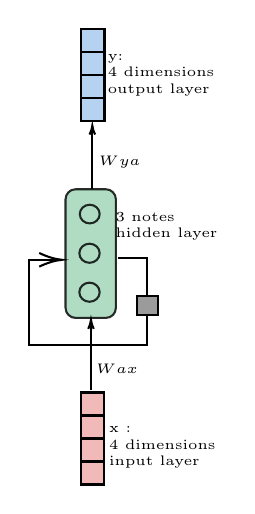
\begin{tikzpicture}[x=0.75pt,y=0.75pt,yscale=-1,xscale=1]
%uncomment if require: \path (0,300); %set diagram left start at 0, and has height of 300

%Rounded Rect [id:dp5767801512845814] 
\draw  [color={rgb, 255:red, 0; green, 0; blue, 0 }  ,draw opacity=0.82 ][fill={rgb, 255:red, 78; green, 178; blue, 121 }  ,fill opacity=0.45 ][line width=0.75]  (117.57,131.31) .. controls (117.57,128.63) and (119.74,126.46) .. (122.42,126.46) -- (136.98,126.46) .. controls (139.66,126.46) and (141.83,128.63) .. (141.83,131.31) -- (141.83,183.6) .. controls (141.83,186.28) and (139.66,188.46) .. (136.98,188.46) -- (122.42,188.46) .. controls (119.74,188.46) and (117.57,186.28) .. (117.57,183.6) -- cycle ;
%Shape: Ellipse [id:dp18804427153778946] 
\draw  [color={rgb, 255:red, 0; green, 0; blue, 0 }  ,draw opacity=0.82 ] (124.44,138.43) .. controls (124.44,135.95) and (126.58,133.93) .. (129.23,133.93) .. controls (131.88,133.93) and (134.02,135.95) .. (134.02,138.43) .. controls (134.02,140.91) and (131.88,142.92) .. (129.23,142.92) .. controls (126.58,142.92) and (124.44,140.91) .. (124.44,138.43) -- cycle ;
%Shape: Ellipse [id:dp672728185189052] 
\draw  [color={rgb, 255:red, 0; green, 0; blue, 0 }  ,draw opacity=0.82 ] (124.22,176.07) .. controls (124.22,173.53) and (126.41,171.47) .. (129.12,171.47) .. controls (131.83,171.47) and (134.02,173.53) .. (134.02,176.07) .. controls (134.02,178.61) and (131.83,180.67) .. (129.12,180.67) .. controls (126.41,180.67) and (124.22,178.61) .. (124.22,176.07) -- cycle ;
%Shape: Ellipse [id:dp22457931655016228] 
\draw  [color={rgb, 255:red, 0; green, 0; blue, 0 }  ,draw opacity=0.82 ] (124.22,157.3) .. controls (124.22,154.76) and (126.41,152.7) .. (129.12,152.7) .. controls (131.83,152.7) and (134.02,154.76) .. (134.02,157.3) .. controls (134.02,159.84) and (131.83,161.9) .. (129.12,161.9) .. controls (126.41,161.9) and (124.22,159.84) .. (124.22,157.3) -- cycle ;
%Shape: Rectangle [id:dp3603601739458042] 
\draw  [fill={rgb, 255:red, 234; green, 141; blue, 141 }  ,fill opacity=0.61 ] (124.9,224.38) -- (136.12,224.38) -- (136.12,235.47) -- (124.9,235.47) -- cycle ;
%Shape: Rectangle [id:dp3229189908551803] 
\draw  [fill={rgb, 255:red, 234; green, 141; blue, 141 }  ,fill opacity=0.61 ] (124.9,235.47) -- (136.12,235.47) -- (136.12,246.56) -- (124.9,246.56) -- cycle ;
%Shape: Rectangle [id:dp21435953126093987] 
\draw  [fill={rgb, 255:red, 234; green, 141; blue, 141 }  ,fill opacity=0.61 ] (124.9,246.56) -- (136.12,246.56) -- (136.12,257.64) -- (124.9,257.64) -- cycle ;
%Shape: Rectangle [id:dp23717670155716364] 
\draw  [fill={rgb, 255:red, 234; green, 141; blue, 141 }  ,fill opacity=0.61 ] (124.9,257.64) -- (136.12,257.64) -- (136.12,268.73) -- (124.9,268.73) -- cycle ;

%Shape: Rectangle [id:dp5297698591025225] 
\draw  [fill={rgb, 255:red, 148; green, 188; blue, 234 }  ,fill opacity=0.68 ] (125.11,49.12) -- (136.33,49.12) -- (136.33,60.21) -- (125.11,60.21) -- cycle ;
%Shape: Rectangle [id:dp38660215409167686] 
\draw  [fill={rgb, 255:red, 148; green, 188; blue, 234 }  ,fill opacity=0.68 ] (125.11,60.21) -- (136.33,60.21) -- (136.33,71.3) -- (125.11,71.3) -- cycle ;
%Shape: Rectangle [id:dp69064370761254] 
\draw  [fill={rgb, 255:red, 148; green, 188; blue, 234 }  ,fill opacity=0.68 ] (125.11,71.3) -- (136.33,71.3) -- (136.33,82.39) -- (125.11,82.39) -- cycle ;
%Shape: Rectangle [id:dp2596136729141916] 
\draw  [fill={rgb, 255:red, 148; green, 188; blue, 234 }  ,fill opacity=0.68 ] (125.11,82.39) -- (136.33,82.39) -- (136.33,93.48) -- (125.11,93.48) -- cycle ;

%Straight Lines [id:da21936148645185471] 
\draw    (129.83,223.17) -- (129.83,191.38) ;
\draw [shift={(129.83,189.38)}, rotate = 450] [color={rgb, 255:red, 0; green, 0; blue, 0 }  ][line width=0.75]    (4.37,-1.32) .. controls (2.78,-0.56) and (1.32,-0.12) .. (0,0) .. controls (1.32,0.12) and (2.78,0.56) .. (4.37,1.32)   ;
%Straight Lines [id:da5720693198246461] 
\draw    (130.48,126.46) -- (130.48,97.75) ;
\draw [shift={(130.48,95.75)}, rotate = 450] [color={rgb, 255:red, 0; green, 0; blue, 0 }  ][line width=0.75]    (4.37,-1.32) .. controls (2.78,-0.56) and (1.32,-0.12) .. (0,0) .. controls (1.32,0.12) and (2.78,0.56) .. (4.37,1.32)   ;
%Straight Lines [id:da45318748010738064] 
\draw    (142.83,159.46) -- (156.83,159.46) -- (156.83,201.46) -- (99.83,201.46) -- (99.83,160.46) -- (113.83,160.46) ;
\draw [shift={(115.83,160.46)}, rotate = 180] [color={rgb, 255:red, 0; green, 0; blue, 0 }  ][line width=0.75]    (10.93,-3.29) .. controls (6.95,-1.4) and (3.31,-0.3) .. (0,0) .. controls (3.31,0.3) and (6.95,1.4) .. (10.93,3.29)   ;
%Shape: Rectangle [id:dp46321775555410516] 
\draw  [fill={rgb, 255:red, 155; green, 155; blue, 155 }  ,fill opacity=1 ] (151.83,177.79) -- (162.25,177.79) -- (162.25,186.96) -- (151.83,186.96) -- cycle ;

% Text Node
\draw (164.21,251) node  [font=\tiny,color={rgb, 255:red, 0; green, 0; blue, 0 }  ,opacity=1 ] [align=left] {x :\\4 dimensions\\input layer};
% Text Node
\draw (163.57,71.49) node  [font=\tiny,color={rgb, 255:red, 0; green, 0; blue, 0 }  ,opacity=1 ] [align=left] {y:\\4 dimensions\\output layer};
% Text Node
\draw (166.21,144.37) node  [font=\tiny,color={rgb, 255:red, 0; green, 0; blue, 0 }  ,opacity=1 ] [align=left] {3 notes\\hidden layer};
% Text Node
\draw (130.83,209.27) node [anchor=north west][inner sep=0.75pt]  [font=\tiny] [align=left] {$\displaystyle Wax$};
% Text Node
\draw (132.16,109.17) node [anchor=north west][inner sep=0.75pt]  [font=\tiny] [align=left] {$\displaystyle Wya$};


\end{tikzpicture}

    \end{center}
    \caption{Sơ đồ tính toán RNN rút gọn}
    \label{folding}
\end{figure}

Bắt đầu tính toán ta cần khởi tạo các ma trận \wax, \waa, \wya \space với các giá trị ngẫu nhiên:

$W_{ax} =
\begin{pmatrix}
0.1 & 0.3 & 0.2 & 0.3\\
0.1 & 0.7 & 0.3 & 0.2\\
0.4 & 0.5 & 0.8 & 0.6\\
0.5 & 0.5 & 0.5 & 0.5
\end{pmatrix} $,

$W_{aa} =
\begin{pmatrix}
0.3 & 0.8 & 0.2 \\
0.6 & 0.4 & 0.1 \\
0.4 & 0.3 & 0.9
\end{pmatrix} $,

$W_{ya} =
\begin{pmatrix}
0.4 & 0.2 & 0.6\\
0.9 & 0.1 & 0.5\\
0.2 & 0.2 & 0.6\\
0.1 & 0.8 & 0.4
\end{pmatrix}$,

Như đã trình bày ở phần trước, tại bước thứ \textit{t} đầu vào $x^{<t>}$ sẽ được kết hợp với các nút ở lớp ẩn $a^{<t-1>}$ bằng hàm $g_{1}$ (thường dùng là \textit{tanh} hoặc \textit{ReLU}) để tính toán ra \a{t} và từ \a{t} sẽ tính ra được \y{t} thông qua hàm $g_{2}$ (thường là hàm \textit{softmax} hoặc hàm \textit{sigmoid} tùy theo số phân lớp, ở đây ta sẽ dùng \textit{softmax} vì giá trị đầu ra \y{t} có 4 chiều). Quá trình này lặp lại như sau:

\textbf{Bước lan truyền thuận:}

Giá trị \a{0} được lấy tùy ý, ví dụ, \a{0} = $\begin{pmatrix} 0 & 0 & 0 \end{pmatrix} ^{T}$,  ký tự đầu vào \x{1} = $H$ =  $\begin{pmatrix} 1 & 0 & 0 & 0 \end{pmatrix} ^{T} $, ta tính được $a^{<1>}$, $\widehat{y}^{<1>}$:

\begin{equation*}
    \begin{split}
    a^{<1>} & = g_{1}(W_{aa}a^{<0>} + W_{ax}x^{<1>} + b_{a}) \\
     & = tanh ( \space
        \begin{pmatrix} .3 & .8 & .2 \\  .6 & .4 & .1 \\ .4 & .3 & .9 \end{pmatrix}
        \begin{pmatrix}0\\0\\0\end{pmatrix} +
        \begin{pmatrix}.1 & .3 & .2 & .3\\ .1 & .7 & .3 & .2\\.4 & .5 & .8 & .6\end{pmatrix}
        \begin{pmatrix} 1 \\ 0 \\ 0 \\ 0 \end{pmatrix}
        + 0.6 \space  )\\
     & = tanh( \begin{pmatrix}  .7 \\ .7 \\ 1. \end{pmatrix} ) \\
     & = \begin{pmatrix} .6 \\ .6 \\ .76 \end{pmatrix}
    \end{split}
\end{equation*}

\begin{equation*}
    \begin{split}
    \widehat{y}^{<1>} & = g_{2}(W_{ya}a^{<1>} + b_{y}) \\
     & = softmax(
     \begin{pmatrix}.4 & .2 & .6\\
                    .9 & .1 & .5\\
                    .2 & .2 & .6\\
                    .1 & .8 & .4  \end{pmatrix}
     \begin{pmatrix} .6 \\ .6 \\ .76 \end{pmatrix}
     + .6 )\\
     & = \begin{pmatrix} .24 \\ .29 \\ .21 \\ .26 \end{pmatrix}
    \end{split}
\end{equation*}

Tiếp tục sử dụng tính toán tương tự ta tính được:
\begin{equation*}
    \begin{split}
    a^{<2>} & =  \begin{pmatrix}.94 & .96 &.98 \end{pmatrix}^{T} \\
    \widehat{y}^{<2>} & = \begin{pmatrix}.23 & .33 & .18 & .25 \end{pmatrix}^{T}
    \end{split}
\end{equation*}

Tóm lại ta có \textit{sơ đồ tính toán (computational graph)} như hình dưới đây cho bước lan truyền thuận:
\begin{figure}[!h]
    \begin{center}
        

\tikzset{every picture/.style={line width=0.75pt}} %set default line width to 0.75pt        

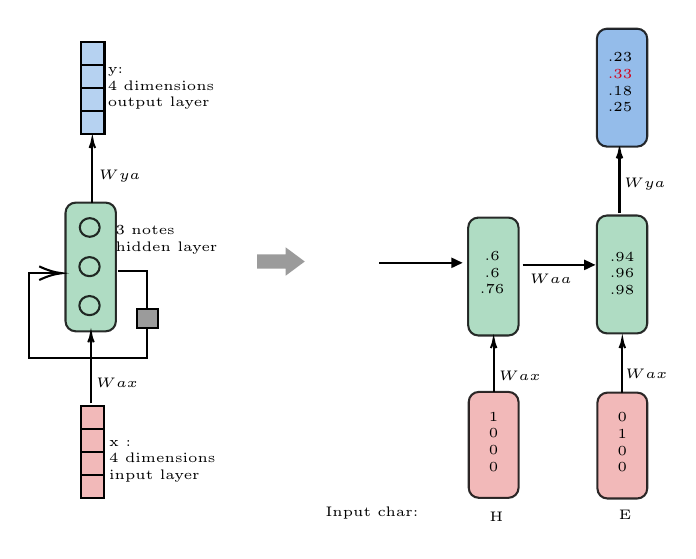
\begin{tikzpicture}[x=0.75pt,y=0.75pt,yscale=-1,xscale=1]
%uncomment if require: \path (0,300); %set diagram left start at 0, and has height of 300

%Rounded Rect [id:dp5767801512845814] 
\draw  [color={rgb, 255:red, 0; green, 0; blue, 0 }  ,draw opacity=0.82 ][fill={rgb, 255:red, 78; green, 178; blue, 121 }  ,fill opacity=0.45 ][line width=0.75]  (117.57,131.31) .. controls (117.57,128.63) and (119.74,126.46) .. (122.42,126.46) -- (136.98,126.46) .. controls (139.66,126.46) and (141.83,128.63) .. (141.83,131.31) -- (141.83,183.6) .. controls (141.83,186.28) and (139.66,188.46) .. (136.98,188.46) -- (122.42,188.46) .. controls (119.74,188.46) and (117.57,186.28) .. (117.57,183.6) -- cycle ;
%Straight Lines [id:da08198893479819136] 
\draw    (323.83,217.67) -- (323.83,194.17) ;
\draw [shift={(323.83,192.17)}, rotate = 450] [color={rgb, 255:red, 0; green, 0; blue, 0 }  ][line width=0.75]    (4.37,-1.32) .. controls (2.78,-0.56) and (1.32,-0.12) .. (0,0) .. controls (1.32,0.12) and (2.78,0.56) .. (4.37,1.32)   ;
%Straight Lines [id:da27259750014998585] 
\draw    (337.83,156.46) -- (369.83,156.46) ;
\draw [shift={(372.83,156.46)}, rotate = 180] [fill={rgb, 255:red, 0; green, 0; blue, 0 }  ][line width=0.08]  [draw opacity=0] (5.36,-2.57) -- (0,0) -- (5.36,2.57) -- cycle    ;
%Straight Lines [id:da14030301096924913] 
\draw    (384.48,131.46) -- (384.48,102.75) ;
\draw [shift={(384.48,100.75)}, rotate = 450] [color={rgb, 255:red, 0; green, 0; blue, 0 }  ][line width=0.75]    (4.37,-1.32) .. controls (2.78,-0.56) and (1.32,-0.12) .. (0,0) .. controls (1.32,0.12) and (2.78,0.56) .. (4.37,1.32)   ;
%Straight Lines [id:da5186597746729542] 
\draw    (268.83,155.46) -- (305.83,155.46) ;
\draw [shift={(308.83,155.46)}, rotate = 180] [fill={rgb, 255:red, 0; green, 0; blue, 0 }  ][line width=0.08]  [draw opacity=0] (5.36,-2.57) -- (0,0) -- (5.36,2.57) -- cycle    ;
%Right Arrow [id:dp4588186786561803] 
\draw  [draw opacity=0][fill={rgb, 255:red, 155; green, 155; blue, 155 }  ,fill opacity=1 ] (209.83,151.42) -- (223.63,151.42) -- (223.63,148) -- (232.83,154.83) -- (223.63,161.67) -- (223.63,158.25) -- (209.83,158.25) -- cycle ;
%Straight Lines [id:da49006821221672503] 
% \draw    (398.83,156.46) -- (432.83,156.46) ;
% \draw [shift={(435.83,156.46)}, rotate = 180] [fill={rgb, 255:red, 0; green, 0; blue, 0 }  ][line width=0.08]  [draw opacity=0] (5.36,-2.57) -- (0,0) -- (5.36,2.57) -- cycle    ;
%Shape: Ellipse [id:dp18804427153778946] 
\draw  [color={rgb, 255:red, 0; green, 0; blue, 0 }  ,draw opacity=0.82 ] (124.44,138.43) .. controls (124.44,135.95) and (126.58,133.93) .. (129.23,133.93) .. controls (131.88,133.93) and (134.02,135.95) .. (134.02,138.43) .. controls (134.02,140.91) and (131.88,142.92) .. (129.23,142.92) .. controls (126.58,142.92) and (124.44,140.91) .. (124.44,138.43) -- cycle ;
%Shape: Ellipse [id:dp672728185189052] 
\draw  [color={rgb, 255:red, 0; green, 0; blue, 0 }  ,draw opacity=0.82 ] (124.22,176.07) .. controls (124.22,173.53) and (126.41,171.47) .. (129.12,171.47) .. controls (131.83,171.47) and (134.02,173.53) .. (134.02,176.07) .. controls (134.02,178.61) and (131.83,180.67) .. (129.12,180.67) .. controls (126.41,180.67) and (124.22,178.61) .. (124.22,176.07) -- cycle ;
%Shape: Ellipse [id:dp22457931655016228] 
\draw  [color={rgb, 255:red, 0; green, 0; blue, 0 }  ,draw opacity=0.82 ] (124.22,157.3) .. controls (124.22,154.76) and (126.41,152.7) .. (129.12,152.7) .. controls (131.83,152.7) and (134.02,154.76) .. (134.02,157.3) .. controls (134.02,159.84) and (131.83,161.9) .. (129.12,161.9) .. controls (126.41,161.9) and (124.22,159.84) .. (124.22,157.3) -- cycle ;
%Shape: Rectangle [id:dp3603601739458042] 
\draw  [fill={rgb, 255:red, 234; green, 141; blue, 141 }  ,fill opacity=0.61 ] (124.9,224.38) -- (136.12,224.38) -- (136.12,235.47) -- (124.9,235.47) -- cycle ;
%Shape: Rectangle [id:dp3229189908551803] 
\draw  [fill={rgb, 255:red, 234; green, 141; blue, 141 }  ,fill opacity=0.61 ] (124.9,235.47) -- (136.12,235.47) -- (136.12,246.56) -- (124.9,246.56) -- cycle ;
%Shape: Rectangle [id:dp21435953126093987] 
\draw  [fill={rgb, 255:red, 234; green, 141; blue, 141 }  ,fill opacity=0.61 ] (124.9,246.56) -- (136.12,246.56) -- (136.12,257.64) -- (124.9,257.64) -- cycle ;
%Shape: Rectangle [id:dp23717670155716364] 
\draw  [fill={rgb, 255:red, 234; green, 141; blue, 141 }  ,fill opacity=0.61 ] (124.9,257.64) -- (136.12,257.64) -- (136.12,268.73) -- (124.9,268.73) -- cycle ;

%Shape: Rectangle [id:dp5297698591025225] 
\draw  [fill={rgb, 255:red, 148; green, 188; blue, 234 }  ,fill opacity=0.68 ] (125.11,49.12) -- (136.33,49.12) -- (136.33,60.21) -- (125.11,60.21) -- cycle ;
%Shape: Rectangle [id:dp38660215409167686] 
\draw  [fill={rgb, 255:red, 148; green, 188; blue, 234 }  ,fill opacity=0.68 ] (125.11,60.21) -- (136.33,60.21) -- (136.33,71.3) -- (125.11,71.3) -- cycle ;
%Shape: Rectangle [id:dp69064370761254] 
\draw  [fill={rgb, 255:red, 148; green, 188; blue, 234 }  ,fill opacity=0.68 ] (125.11,71.3) -- (136.33,71.3) -- (136.33,82.39) -- (125.11,82.39) -- cycle ;
%Shape: Rectangle [id:dp2596136729141916] 
\draw  [fill={rgb, 255:red, 148; green, 188; blue, 234 }  ,fill opacity=0.68 ] (125.11,82.39) -- (136.33,82.39) -- (136.33,93.48) -- (125.11,93.48) -- cycle ;

%Straight Lines [id:da21936148645185471] 
\draw    (129.83,223.17) -- (129.83,191.38) ;
\draw [shift={(129.83,189.38)}, rotate = 450] [color={rgb, 255:red, 0; green, 0; blue, 0 }  ][line width=0.75]    (4.37,-1.32) .. controls (2.78,-0.56) and (1.32,-0.12) .. (0,0) .. controls (1.32,0.12) and (2.78,0.56) .. (4.37,1.32)   ;
%Straight Lines [id:da5720693198246461] 
\draw    (130.48,126.46) -- (130.48,97.75) ;
\draw [shift={(130.48,95.75)}, rotate = 450] [color={rgb, 255:red, 0; green, 0; blue, 0 }  ][line width=0.75]    (4.37,-1.32) .. controls (2.78,-0.56) and (1.32,-0.12) .. (0,0) .. controls (1.32,0.12) and (2.78,0.56) .. (4.37,1.32)   ;
%Straight Lines [id:da45318748010738064] 
\draw    (142.83,159.46) -- (156.83,159.46) -- (156.83,201.46) -- (99.83,201.46) -- (99.83,160.46) -- (113.83,160.46) ;
\draw [shift={(115.83,160.46)}, rotate = 180] [color={rgb, 255:red, 0; green, 0; blue, 0 }  ][line width=0.75]    (10.93,-3.29) .. controls (6.95,-1.4) and (3.31,-0.3) .. (0,0) .. controls (3.31,0.3) and (6.95,1.4) .. (10.93,3.29)   ;
%Shape: Rectangle [id:dp46321775555410516] 
\draw  [fill={rgb, 255:red, 155; green, 155; blue, 155 }  ,fill opacity=1 ] (151.83,177.79) -- (162.25,177.79) -- (162.25,186.96) -- (151.83,186.96) -- cycle ;
%Rounded Rect [id:dp9185519263132114] 
\draw  [color={rgb, 255:red, 0; green, 0; blue, 0 }  ,draw opacity=0.82 ][fill={rgb, 255:red, 78; green, 178; blue, 121 }  ,fill opacity=0.45 ][line width=0.75]  (311.57,138.52) .. controls (311.57,135.84) and (313.74,133.67) .. (316.42,133.67) -- (330.98,133.67) .. controls (333.66,133.67) and (335.83,135.84) .. (335.83,138.52) -- (335.83,185.6) .. controls (335.83,188.28) and (333.66,190.46) .. (330.98,190.46) -- (316.42,190.46) .. controls (313.74,190.46) and (311.57,188.28) .. (311.57,185.6) -- cycle ;
%Rounded Rect [id:dp7418323406917965] 
\draw  [color={rgb, 255:red, 0; green, 0; blue, 0 }  ,draw opacity=0.82 ][fill={rgb, 255:red, 78; green, 178; blue, 121 }  ,fill opacity=0.45 ][line width=0.75]  (373.57,137.52) .. controls (373.57,134.84) and (375.74,132.67) .. (378.42,132.67) -- (392.98,132.67) .. controls (395.66,132.67) and (397.83,134.84) .. (397.83,137.52) -- (397.83,184.6) .. controls (397.83,187.28) and (395.66,189.46) .. (392.98,189.46) -- (378.42,189.46) .. controls (375.74,189.46) and (373.57,187.28) .. (373.57,184.6) -- cycle ;
%Rounded Rect [id:dp3739746455078473] 
\draw  [color={rgb, 255:red, 0; green, 0; blue, 0 }  ,draw opacity=0.82 ][fill={rgb, 255:red, 148; green, 188; blue, 234 }  ,fill opacity=1 ][line width=0.75]  (373.57,47.52) .. controls (373.57,44.84) and (375.74,42.67) .. (378.42,42.67) -- (392.98,42.67) .. controls (395.66,42.67) and (397.83,44.84) .. (397.83,47.52) -- (397.83,94.6) .. controls (397.83,97.28) and (395.66,99.46) .. (392.98,99.46) -- (378.42,99.46) .. controls (375.74,99.46) and (373.57,97.28) .. (373.57,94.6) -- cycle ;
%Rounded Rect [id:dp8951478388246187] 
\draw  [color={rgb, 255:red, 0; green, 0; blue, 0 }  ,draw opacity=0.82 ][fill={rgb, 255:red, 234; green, 141; blue, 141 }  ,fill opacity=0.61 ][line width=0.75]  (311.83,222.47) .. controls (311.83,219.82) and (313.98,217.67) .. (316.63,217.67) -- (331.03,217.67) .. controls (333.68,217.67) and (335.83,219.82) .. (335.83,222.47) -- (335.83,263.87) .. controls (335.83,266.52) and (333.68,268.67) .. (331.03,268.67) -- (316.63,268.67) .. controls (313.98,268.67) and (311.83,266.52) .. (311.83,263.87) -- cycle ;
%Straight Lines [id:da83582986868796] 
\draw    (385.83,218) -- (385.83,194.17) ;
\draw [shift={(385.83,192.17)}, rotate = 450] [color={rgb, 255:red, 0; green, 0; blue, 0 }  ][line width=0.75]    (4.37,-1.32) .. controls (2.78,-0.56) and (1.32,-0.12) .. (0,0) .. controls (1.32,0.12) and (2.78,0.56) .. (4.37,1.32)   ;
%Rounded Rect [id:dp20838548651521271] 
\draw  [color={rgb, 255:red, 0; green, 0; blue, 0 }  ,draw opacity=0.82 ][fill={rgb, 255:red, 234; green, 141; blue, 141 }  ,fill opacity=0.61 ][line width=0.75]  (373.83,222.8) .. controls (373.83,220.15) and (375.98,218) .. (378.63,218) -- (393.03,218) .. controls (395.68,218) and (397.83,220.15) .. (397.83,222.8) -- (397.83,264.2) .. controls (397.83,266.85) and (395.68,269) .. (393.03,269) -- (378.63,269) .. controls (375.98,269) and (373.83,266.85) .. (373.83,264.2) -- cycle ;

% Text Node
\draw  [draw opacity=0]  (321.83,202.02) -- (344.83,202.02) -- (344.83,216.02) -- (321.83,216.02) -- cycle  ;
\draw (324.83,206.02) node [anchor=north west][inner sep=0.75pt]  [font=\tiny] [align=left] {$\displaystyle Wax$};
% Text Node
\draw  [draw opacity=0]  (382.16,109.17) -- (405.16,109.17) -- (405.16,123.17) -- (382.16,123.17) -- cycle  ;
\draw (385.16,113.17) node [anchor=north west][inner sep=0.75pt]  [font=\tiny] [align=left] {$\displaystyle Wya$};
% Text Node
\draw (323.13,160.32) node  [font=\tiny ] [align=left] {\begin{minipage}[lt]{9.520000000000001pt}\setlength\topsep{0pt}
\begin{center}
{\tiny .6}\\{\tiny .6}\\{\tiny .76}
\end{center}

\end{minipage}};
% Text Node
\draw (164.21,251) node  [font=\tiny,color={rgb, 255:red, 0; green, 0; blue, 0 }  ,opacity=1 ] [align=left] {x :\\4 dimensions\\input layer};
% Text Node
\draw (163.57,71.49) node  [font=\tiny,color={rgb, 255:red, 0; green, 0; blue, 0 }  ,opacity=1 ] [align=left] {y:\\4 dimensions\\output layer};
% Text Node
\draw (166.21,144.37) node  [font=\tiny,color={rgb, 255:red, 0; green, 0; blue, 0 }  ,opacity=1 ] [align=left] {3 notes\\hidden layer};
% Text Node
\draw (130.83,209.27) node [anchor=north west][inner sep=0.75pt]  [font=\tiny] [align=left] {$\displaystyle Wax$};
% Text Node
\draw (132.16,109.17) node [anchor=north west][inner sep=0.75pt]  [font=\tiny] [align=left] {$\displaystyle Wya$};
% Text Node
\draw (385.7,160.46) node  [font=\tiny] [align=left] {\begin{minipage}[lt]{9.520000000000001pt}\setlength\topsep{0pt}
\begin{center}
{\tiny .94}\\{\tiny .96}\\{\tiny .98}
\end{center}

\end{minipage}};
% Text Node
\draw (384.7,68.46) node  [font=\tiny] [align=left] {\begin{minipage}[lt]{9.100644pt}\setlength\topsep{0pt}
\begin{center}
{\tiny .23}\\{\tiny \textcolor[rgb]{0.82,0.01,0.11}{.33}}\\{\tiny .18}\\{\tiny .25}
\end{center}

\end{minipage}};
% Text Node
\draw (323.83,241.67) node  [font=\tiny] [align=left] {\begin{minipage}[lt]{8.67pt}\setlength\topsep{0pt}
\begin{center}
{\tiny 1}\\{\tiny 0}\\{\tiny 0}\\{\tiny 0}
\end{center}

\end{minipage}};
% Text Node
\draw  [draw opacity=0]  (383.83,202.36) -- (406.83,202.36) -- (406.83,216.36) -- (383.83,216.36) -- cycle  ;
\draw (386.83,206.36) node [anchor=north west][inner sep=0pt]  [font=\tiny] [align=left] {$\displaystyle Wax$};
% Text Node
\draw (385.83,242) node  [font=\tiny] [align=left] {\begin{minipage}[lt]{8.67pt}\setlength\topsep{0pt}
\begin{center}
{\tiny 0}\\{\tiny 1}\\{\tiny 0}\\{\tiny 0}
\end{center}

\end{minipage}};
% Text Node
\draw  [draw opacity=0]  (336.83,155.46) -- (359.83,155.46) -- (359.83,169.46) -- (336.83,169.46) -- cycle  ;
\draw (339.83,159.46) node [anchor=north west][inner sep=0.75pt]  [font=\tiny] [align=left] {$\displaystyle Waa$};
% Text Node
\draw (265.21,276) node  [font=\tiny,color={rgb, 255:red, 0; green, 0; blue, 0 }  ,opacity=1 ] [align=left] {Input char:};
% Text Node
\draw (325.21,278) node  [font=\tiny,color={rgb, 255:red, 0; green, 0; blue, 0 }  ,opacity=1 ] [align=left] {H};
% Text Node
\draw (387.21,277) node  [font=\tiny,color={rgb, 255:red, 0; green, 0; blue, 0 }  ,opacity=1 ] [align=left] {E};


\end{tikzpicture}

    \end{center}
    \caption{Sơ đồ tính toán của bài toán dự đoán chữ cái dạng đầy đủ}
\end{figure}

Nếu ta chuyển đổi các xác suất này để hiểu dự đoán, chúng ta sẽ thấy rằng, tại đầu vào thứ 2, $x^{2}$, mô hình nói rằng xác suất cao nhất sẽ xuất hiện tiếp theo là chữ ``E''([0 1 0 0]) vì $\hat{y}^{<2>}$ =[.23  .33  .18  .25]. Điều đó cho thấy, với hệ thống hiện tại, máy sẽ dự đoán chữ tiếp theo sau khi nhập ``HE'’ sẽ là chữ ``E'' chứ không phải chữ ``L'' như mong muốn.

Đó là vì ta chưa thực hiện cho máy học. Ở bước lan truyền ngược, ta cập nhật các thông số \wax, \waa, \wya, \ba, \by \space sao cho tối thiểu hàm mất mát.\\

\textbf{Bước lan truyền ngược:}

Ta viết lại các ma trận trọng số để cập nhật các bias \ba và \by cùng lúc với \wax và \wya:

\begin{equation*}
W_{ax} \longrightarrow (W_{ax} \mid b_a) \longrightarrow \begin{pmatrix} 0.1 & 0.3 & 0.2 & 0.3 & 0.6\\0.1 & 0.7 & 0.3 & 0.2 & 0.6\\0.4 & 0.5 & 0.8 & 0.6 & 0.6 \end{pmatrix}
\end{equation*}

Chọn hệ số học $\eta$ = 1.0, cập nhật $W_{ax}$ theo công thức:\\
\begin{equation*}
    \begin{split}
    W_{ya} & = W_{ya} - \eta (\widehat{y}^{<2>} - y^{<2>}) \otimes a^{<2>} \\
     & = \begin{pmatrix}0.4 & 0.2 & 0.6 & 0.6\\0.9 & 0.1 & 0.5 & 0.6\\ 0.2 & 0.2 & 0.6 & 0.6 \\0.1 & 0.8 & 0.4 & 0.6\end{pmatrix} - 1.0 (\begin{pmatrix}.23\\.33\\.18\\.25 \end{pmatrix}-
    \begin{pmatrix}0\\0\\1\\0\end{pmatrix}) \otimes \begin{pmatrix}.94\\.96\\.98\\1 \end{pmatrix} \\
     & = \begin{pmatrix}0.4 & 0.2 & 0.6 & 0.6\\0.9 & 0.1 & 0.5 & 0.6\\ 0.2 & 0.2 & 0.6 & 0.6 \\0.1 & 0.8 & 0.4 & 0.6\end{pmatrix} - \begin{pmatrix}0.2162 & 0.2208 & 0.2254 & 0.23\\0.3102 & 0.3168 & 0.3234 & 0.33\\ -0.7708 & -0.7872 & -0.8036 & -0.82 \\0.235 & 0.24 & 0.245 & 0.25 \end{pmatrix} \\
     & = \begin{pmatrix}0.1838 & -0.0208 & 0.3746 & 0.37\\0.5898 & -0.2168 & 0.1766 & 0.27\\ 0.9708 & 0.9872 & 1.4036 & 1.42 \\-0.135 & 0.56 & 0.155 & 0.35 \end{pmatrix}
    \end{split}
\end{equation*}

Tương tự ta cập nhật $W_{ax}$ và $W_{aa}$. Sau một số lần lặp đủ lớn ta thu được bộ tham số $(W, b)$ có thể sử dụng làm mô hình dự đoán. Đầu ra $\widehat{y}^{<t>}$ chính là giá trị dự đoán sau khi có \textit{t} kí tự được nhập.

\newpage
\section{Bài tập}
\begin{exer}
Nhận diện sequence data:

Trong các ngữ cảnh sau đây, dữ liệu nào thuộc về dạng sequence data? Tại sao?
    \begin{enumerate}[label=\alph*)]
    \item Dữ liệu chứng khoán: dữ liệu về giá các mã cổ phiếu bao gồm loại mã, giá mở cửa, giá đóng cửa của một sàn chứng khoán được thu thập liên tục theo thời gian.
    \item Dữ liệu về thời tiết: thông tin khí tượng thu thập được theo vùng miền về nhiệt độ, độ ẩm, lượng mưa, ...
    \item Dữ liệu về chuỗi văn bản: một lượng lớn văn bản bao gồm nhiều câu ở một ngôn ngữ nào đó
    \end{enumerate}
\end{exer}

\begin{exer}
Nhận dạng và phân tích dạng bài toán:

Với các bài toán cụ thể sau đây, có thể mô hình hóa chúng để áp dụng RNN được không? Nếu có, hãy xếp dạng bài toán vào một dạng của RNN (one-to-many, many-to-one, many-to-many, sequence-to-sequence) và giải thích.
    \begin{enumerate}[label=\alph*)]
    \item Bài toán về Language model: Dự đoán kí tự hoặc từ tiếp theo xuất hiện trong một chuỗi văn bản đang nhập.
    \item Bài toán dự báo thời tiết: Dự đoán thời tiết cho chiều hôm nay dựa vào các thông số khí tượng hiện có và thông tin thời tiết từ các ngày trước đó.
    \item Dự đoán doanh số bán hàng: dựa vào thông tin doanh số của thời gian hiện tại, liền trước, cùng kì tháng trước, cùng kì quý trước và cùng kì năm trước, hãy dự báo doanh số bán hàng cho từng ngày trong một tháng tới.
    \item Bài toán dịch máy: Từ một câu văn bản ở tiếng Việt, hãy dịch câu đó sang tiếng Anh. Dạng bài toán có giữ nguyên không nếu như hướng tiếp cận là dịch theo cặp từ (word-by-word)?
    \end{enumerate}
\end{exer}

\clearpage
\begin{exer}
Lan truyền xuôi trong RNN:
    \begin{enumerate}[label=\alph*)]
    \item Trong đồ thị tính toán, ý nghĩa của các nút dữ liệu $\symbf x, \symbf a, \symbf y$ là gì? Giải thích ý nghĩa của các ma trận trọng số?
    \item Tại sao trên đồ thị tính toán có nhiều nút R, nhưng chỉ có một bộ trọng số? Việc dùng chung một bộ trọng số cho các nút có tác dụng gì?
    \end{enumerate}
\end{exer}

\begin{exer}
Lan truyền ngược trong RNN:
    \begin{enumerate}[label=\alph*)]
    \item Trong công thức tính đạo hàm, hãy viết dạng (shape) của từng thành phần (số chiều của vector, ma trận, tensor, ...). Các phép nhân trong chain-rule là phép nhân dạng gì?
    Phép nhân đó với tensor nhiều hơn hai chiều được thực hiện như thế nào?
    \item Dựa vào đồ thị tính toán và công thức truy hồi, chứng minh lại công thức tính đạo hàm cho từng bộ tham số trong mạng.
    \item Giải thích hiện tượng vanishing/exploding gradient, tại sao mạng RNN cơ bản không hiệu quả trong việc ghi nhớ chuỗi dữ liệu dài? Vanishing/exploding gradient sẽ xảy ra với bộ trọng số cụ thể nào trong mạng?
    \end{enumerate}
\end{exer}

\begin{exer}
\leavevmode
    \begin{enumerate}[label=\alph*)]
    \item So sánh RNN và mạng feed-forward truyền thống (MLP là một ví dụ).
    \item Có thể dùng một mạng MLP để biểu diễn chính xác một mạng RNN cơ bản hay không? Nếu có, tại sao không nên dùng?
    \end{enumerate}
\end{exer}

\begin{exer}
Có phải RNN luôn tốt hơn mạng MLP không?
\end{exer}

\clearpage
\begin{exer}
Cho trước một corpus là "Goodbye", với mục tiêu huấn luyện là hệ thống sẽ đoán chữ "d" sau khi người dùng nhập chuỗi "Goo".

Hãy:
    \begin{enumerate}[label=\alph*)]
    \item Tính toán giá trị $\widehat{y}$ và so sánh với kết quả mong muốn khi áp dụng lan truyền xuôi trong RNN. Giải thích kết quả đạt được.
    \item Sử dụng kết quả tính toán được ở câu trên để cập nhật trọng số cho các ma trận trong mạng,biết rằng hệ thống có hệ số học là 0.1 và hàm mất mát là Cross Entropy.
    \end{enumerate}
\end{exer}